\FloatBarrier


\begin{figure}[htbp]
	\begin{minipage}[b]{0.5\textwidth} 
		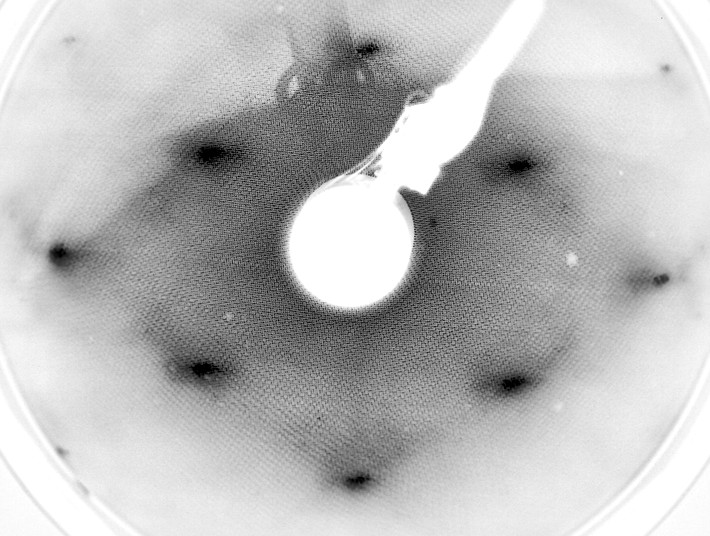
\includegraphics[width=\textwidth]{LEED-Bilder/bearbeitet/unbedampft_E207}
		\label{Bild} 
	\end{minipage}
	\hfill
	\begin{minipage}[b]{0.5\textwidth}
		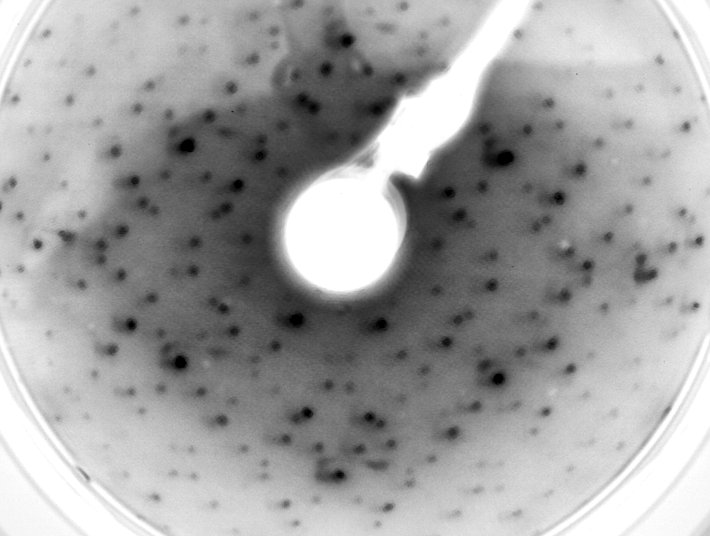
\includegraphics[width=\textwidth]{LEED-Bilder/bearbeitet/unbedampft_E207_MitteKristall.jpg}
		\label{Bild} 
	\end{minipage}
	\caption{Links der Re-Kristall mit scharfen Spots und eindeutiger Struktur. Rechts die
	Re-Oberfläche mit Verschmutzung, zu erkennen an der Überstruktur und den schwächeren Hauptspots.}
\end{figure}

\begin{figure}[htbp]
	\begin{minipage}[b]{0.5\textwidth} 
		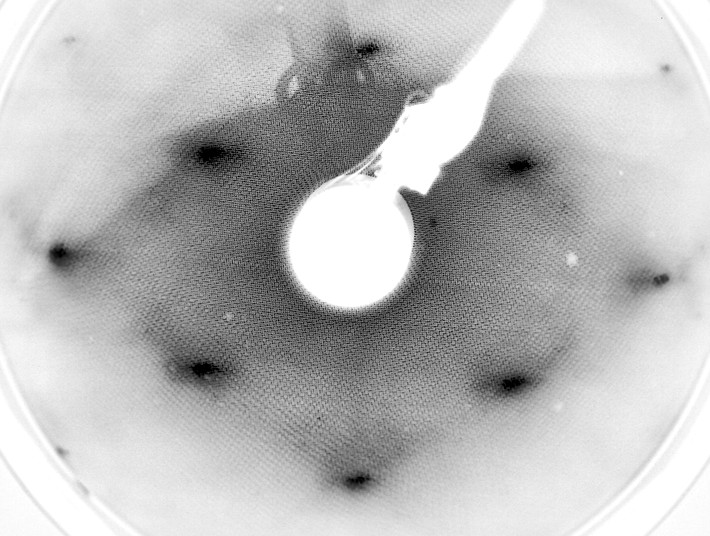
\includegraphics[width=\textwidth]{LEED-Bilder/bearbeitet/unbedampft_E207}
		\caption{Re-Oberfläche}
		\label{Bild} 
	\end{minipage}
	\hfill
	\begin{minipage}[b]{0.5\textwidth}
		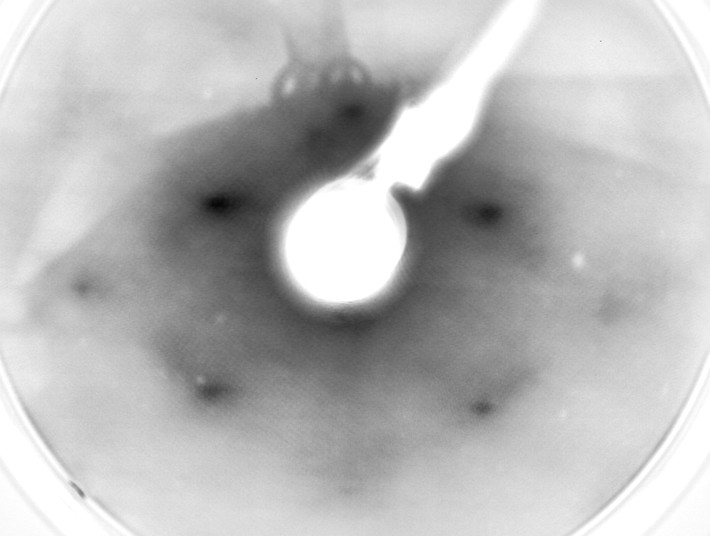
\includegraphics[width=\textwidth]{LEED-Bilder/bearbeitet/0_5ML_E208}
		\caption{1/2 Monolage Au}
		\label{Bild} 
	\end{minipage}
	
	\begin{minipage}[b]{0.5\textwidth} 
		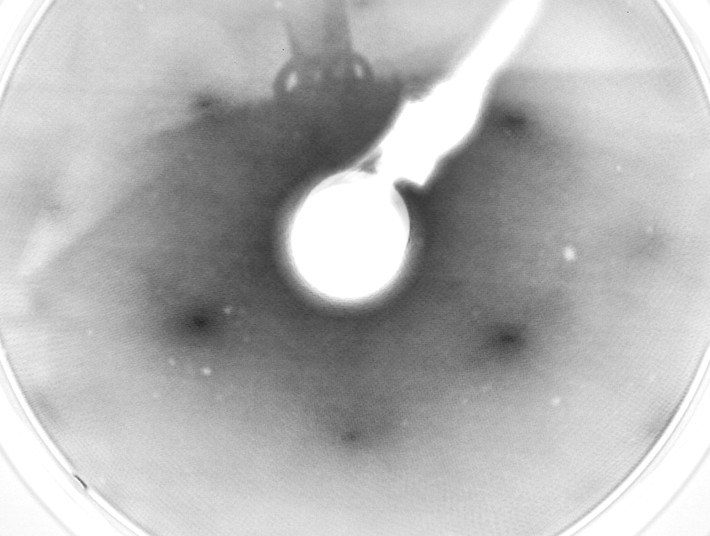
\includegraphics[width=\textwidth]{LEED-Bilder/bearbeitet/1ML_E207}
		\caption{1 Monolage Au}
		\label{Bild} 
	\end{minipage}
	\hfill
	\begin{minipage}[b]{0.5\textwidth}
		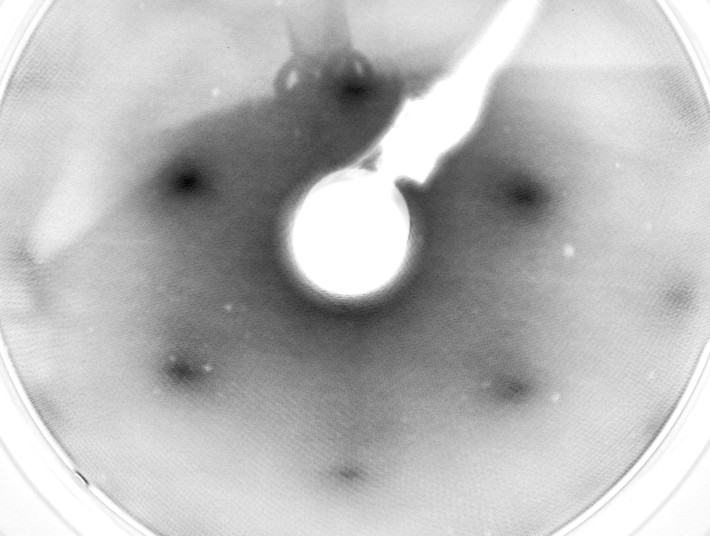
\includegraphics[width=\textwidth]{LEED-Bilder/bearbeitet/6ML_E207}
		\caption{6 Monolagen Au}
		\label{Bild} 
	\end{minipage}
	
	\begin{minipage}[b]{0.5\textwidth} 
		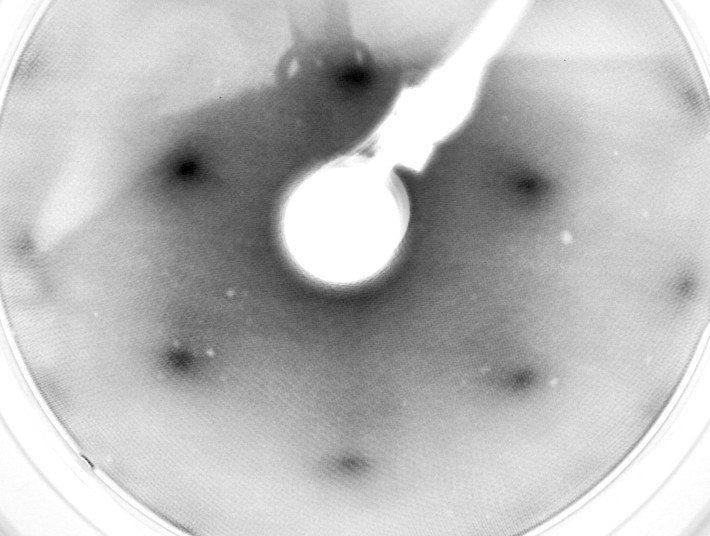
\includegraphics[width=\textwidth]{LEED-Bilder/bearbeitet/10ML_E207}
		\caption{10 Monolagen Au}
		\label{Bild} 
	\end{minipage}
	\hfill
	\begin{minipage}[b]{0.5\textwidth}
		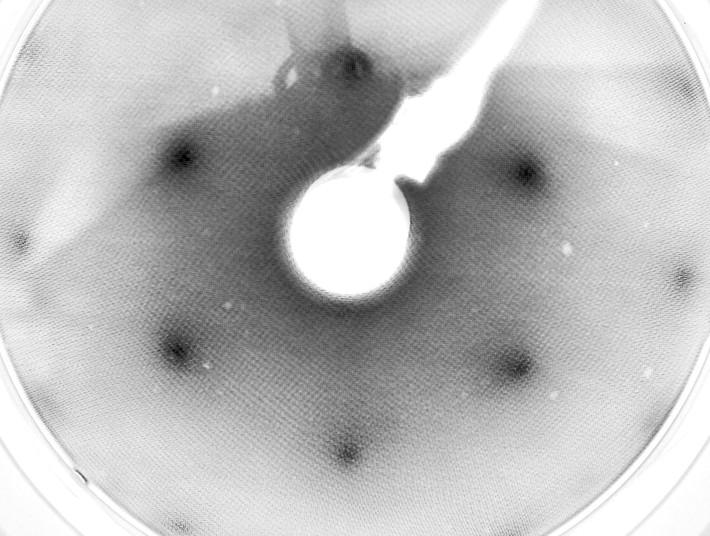
\includegraphics[width=\textwidth]{LEED-Bilder/bearbeitet/30ML_E208}
		\caption{30 Monolagen Au}
		\label{Bild} 
	\end{minipage}
	\caption{noch eine Caption}
\end{figure}


\FloatBarrier